\DiaryEntry{1000 Problems in Probability - 1}{2018-11-15}{Stochastic}

\paragraph{Section 1.3, Problem 1.} We have two events $\Ac, \Bc$ with probabilities $P(\Ac) = 3/4, P(\Bc) = 1/3$. We seek bounds for $P(\Ac \cap \Bc)$ and $P(\Ac \cup \Bc)$.

We first note that $P(\Ac \cap \Bc) = P(\Ac) + P(\Bc) - P(\Ac \cup \Bc)$. If we upper-bound the last term with $1$, we obtain the lower bound

\bee
P(\Ac \cap \Bc) \geq P(\Ac) + P(\Bc) - 1 = \frac{1}{12}
\eee

For the ``other direction'', assume that one set is a subset of the other (e.g. $\Bc$ is a subset of $\Ac$). Then we can lower-bound $P(\Ac \cap \Bc)$ as

\bee
P(\Ac \cap \Bc) \leq \min\{P(\Ac), P(\Bc) \} = \frac{1}{3}
\eee

Combining the two bounds yields

\bee
P(\Ac) + P(\Bc) - 1 \leq P(\Ac \cap \Bc) \leq \min\{P(\Ac), P(\Bc) \}
\eee

An upper bound for $P(\Ac \cup \Bc)$ is obtained by noting that $P(\Ac \cup \Bc) = P(\Ac) + P(\Bc) - P(\Ac \cap \Bc) \leq P(\Ac) + P(\Bc)$. This bound is obtained, when $\Ac$ and $\Bc$ do not overlap. A lower bound is $P(\Ac \cup \Bc) \geq \max\{ P(\Ac), P(\Bc) \}$, obtained when one set is a subset of the other. Combining, we obtain

\bee
\max\{ P(\Ac), P(\Bc) \} \leq P(\Ac \cup \Bc) \leq P(\Ac) + P(\Bc)
\eee

\paragraph{Section 1.7, Problem 1.} Denote a path between $A$ and $B$ via $A \sim B$ and no path via $A \not\sim B$. We have $P(A \not\sim B) = P(B \not\sim C) = p^2$. The required probability is then

\begin{align*}
P(A \sim B | A \not\sim C) = &\frac{P(A \sim B \cap A \not\sim C)}{P(A \not\sim C)} = \frac{P(A \sim B \cap B \not\sim C)}{1 - P(A \sim C)} = \frac{P(A \sim B) P(B \not\sim C)}{1 - P(A \sim B \cap B \sim C)} \\ = & \frac{P(A \sim B) P(B \not\sim C)}{1 - P(A \sim B) P(B \sim C)} = \frac{(1-p^2)p^2}{1-(1-p^2)^2}
\end{align*}

\paragraph{Extension.} Assume we have $n$ different paths linking $A$ and $B$, each failing independently with probability $p_i (i=1...n)$. In oder to calculate the probability that there is no path between $A$ and $B$, we note that this is the probability that all $n$ paths are failing:

\be\label{2018-11-15:eq1}
P(A \not\sim B) = P(\text{link 1 fails} \cap \text{link 2 fails} \cap \cdots \cap \text{link n fails}) = \prod_{i=1}^n p_i
\ee

where we we have used the fact that the failures are independent. The probability for a link between $A$ and $B$ is then $P(A \sim B) = 1 - \prod_{i=1}^n p_i$. Since all $p_i < 1$, the product can be bound by the maximum: $\prod_{i=1}^n p_i \leq \min_i p_i$ and therefore $P(A \sim B) \leq \min_i p_i$. In other words, parallel links always help in increasing reliability. 

Assuming that all $p_i$ are equal $p$, we have

\bee
P(A \sim B) = 1 - p^n
\eee

which is decreasing with $n$.


Now we assume that we have two serial links $A-B-C$ and ask for the probability that there is no connection between $A$ and $C$. Consider $P(A \sim C)$ first,

\be\label{2018-11-15:eq2}
P(A \sim C) = P(A \sim B \cap B \sim C) = P(A \sim B) P(B \sim C)= (1-p_1)(1-p_2)
\ee

where we have used the fact that link failures are independent. Link $A-B$ fails with probability $p_1$ and link $B-C$ fails with probability $p_2$. The probability of failure is $P(A \not\sim C) = 1 - (1-p_1)(1-p_2)$. If $p_1=p_2=p$, we have

\bee
P(A \not\sim C) = 1-(1-p)^2 = 1-1+2p-p^2 \approx 2p, \quad p \ll 1
\eee

For $n$ links in series; i.e.$A_1 - A_2 - \cdots - A_{n+1}$, probability of failure of the whole chain is
\bee
P(A_1 \not\sim A_{n+1}) = 1 - \prod_{i=1}^n (1-p_i) = 1-(1-p)^n \approx n p, \quad p \ll 1
\eee

The product $\prod_{i=1}^n (1-p_i)$ is dominated by the biggest failure probability and $P(A_1 \not\sim A_{n+1}) \leq 1 - \max_i p_i$; i.e. the worst link dominates the overall link failure probability.

\emph{Conclusion} We can easily calculate probabilites of ``union'' events; i.e. $P(\Ec_1 \cap \Ec_2) = P(\Ec_1) P(\Ec_2)$ (whereas $P(\Ec_1 \cup \Ec_2)$ are more difficult). This allows the simple expressions in \eqref{2018-11-15:eq1} and \eqref{2018-11-15:eq2}, but note that \eqref{2018-11-15:eq1} is a failure probability whereas \eqref{2018-11-15:eq2} is a ``success'' probability.

To conclude, consider the example below. The probability for a failure of the $A-B-C$ link is $P = 1 - (1-0.1)(1-10^{-5}) = 0.100008\bar{9}$, clearly dominated by the bad link with failure probability $0.1$. The failure probability considering additionally the parallel link is $P(A \not\sim C) = \left(1 - \left(1 - (1-0.1)(1-10^{-5}\right)\right)10^{-3}\approx 0.000899991$. This probability is largely dominated by the good quality of the direct $A-C$ link.

\vspace{0.5cm}

\SetVertexNormal[Shape = circle, FillColor = orange, LineWidth = 2pt] \SetUpEdge[lw = 1.5pt, color = black, labelcolor = white, labeltext = red, labelstyle = {sloped,draw,text=blue}]

\begin{tikzpicture}

  \Vertex[x=0, y=0]{A}
  \Vertex[x=4, y=0]{B}
  \Vertex[x=8, y=0]{C}
  
  \Edge[label=$0.1$](A)(B)
  \Edge[label=$10^{-5}$](B)(C)
  \tikzset{EdgeStyle/.append style = {bend left}}
  \Edge[label=$10^{-3}$](A)(C)  
  
\end{tikzpicture}


\paragraph{Section 1.8, Problem 1.} Two (fair) dice with probability of one side (per dice) is $1/6$. Probability that $6$ turns up exactely once (a) is given by enumerating all ``good'' cases: $1-6, 2-6, 3-6, 4-6, 5-6, 6-1, 6-2, 6-3, 6-4, 6-5$ and the probability is then $P = 10/36 = 5/18$. For the probability that both numbers are odd (b), note that this happens in $50\%$ of the cases; i.e. $P = 1/2$. The ``good'' cases for throwing a sum of $4$ (c) are $1-3, 2-2, 3-1$ and the probability is $P = 3/36 = 1/12$. Finally, for the ``good'' cases that the sum is divisible by $3$ (d), the relevant sums are $3,6,9,12$. ``Good'' cases yielding a sum of $3$ are $1-2, 2-1$, ``good'' cases for a sum of $6$ are $1-5, 2-4, 3-3, 4-2, 5-1$, ``good'' cases for a sum of $9$ are $3-6, 4-5, 5-4, 6-3$, and finally the ``good'' case for a sum of $12$ is $6-6$. The corresponding probability is then $P = (2 + 5 + 4 + 1)/36 = 12/36 = 1/3$.

\paragraph{Section 1.8, Problem 2.} A fair coin is thrown $n$ times. The probability that - after the $n$-th throw:

\begin{itemize}

\item a head is thrown is $P( n-1 \times T, 1 \times H) = \left(\frac{1}{2}\right)^{n-1} \frac{1}{2} = 2^{-n}$

\item $n/2$ heads and tails have been thrown (assume $n$ even), is $P = {n \choose n/2} 2^{-n/2} 2^{-n/2} = {n \choose n/2}2^{-n}$.

\item exactely two heads have been thrown is $P = {n \choose 2} 2^{-n}$

\item at least two heads have been thrown is $P = 1 - 2^{-n} - {n \choose 1} 2^{-n}$.
  
\end{itemize}


\paragraph{Section 1.8, Problem 29}. An event $A$ is said to be repelled by the event $B$, when $P(A|B) < P(A)$ and to be attracted by $B$, if $P(A|B) > P(A)$. Show that if $B$ attract $A$, then $A$ attracts $B$ and $\bar{B}$ repels $A$.

We have $P(A|B) > P(A) \rightarrow \frac{P(A|B)}{P(A)} = c > 1$ and use Bayes' theorem to calculate

\bee
P(B|A) = \frac{P(A|B)P(B)}{P(A)} = cP(B) > P(B) \qed
\eee

For the second part, we start with $P(B|A)>P(B)$ and $1 - P(\bar{B}|A) = P(B|A) > P(B)$. We can write this as $P(\bar{B}|A) < 1-P(B) = P(\bar{B})$. Using Bayes' theorem, we have

\bee
P(\bar{B}|A) = \frac{P(A|\bar{B})P(\bar{B})}{P(A)} < P(\bar{B})
\eee

From this follows, that $\frac{P(A|\bar{B})}{P(A)} < 1 \rightarrow P(A|\bar{B}) < P(A)$. \qed

%%% Local Variables:
%%% mode: latex
%%% TeX-master: "journal"
%%% End:
